\saveSpaceSec
\section{Experiments}
\begin{figure*}[!t]
\begin{center}
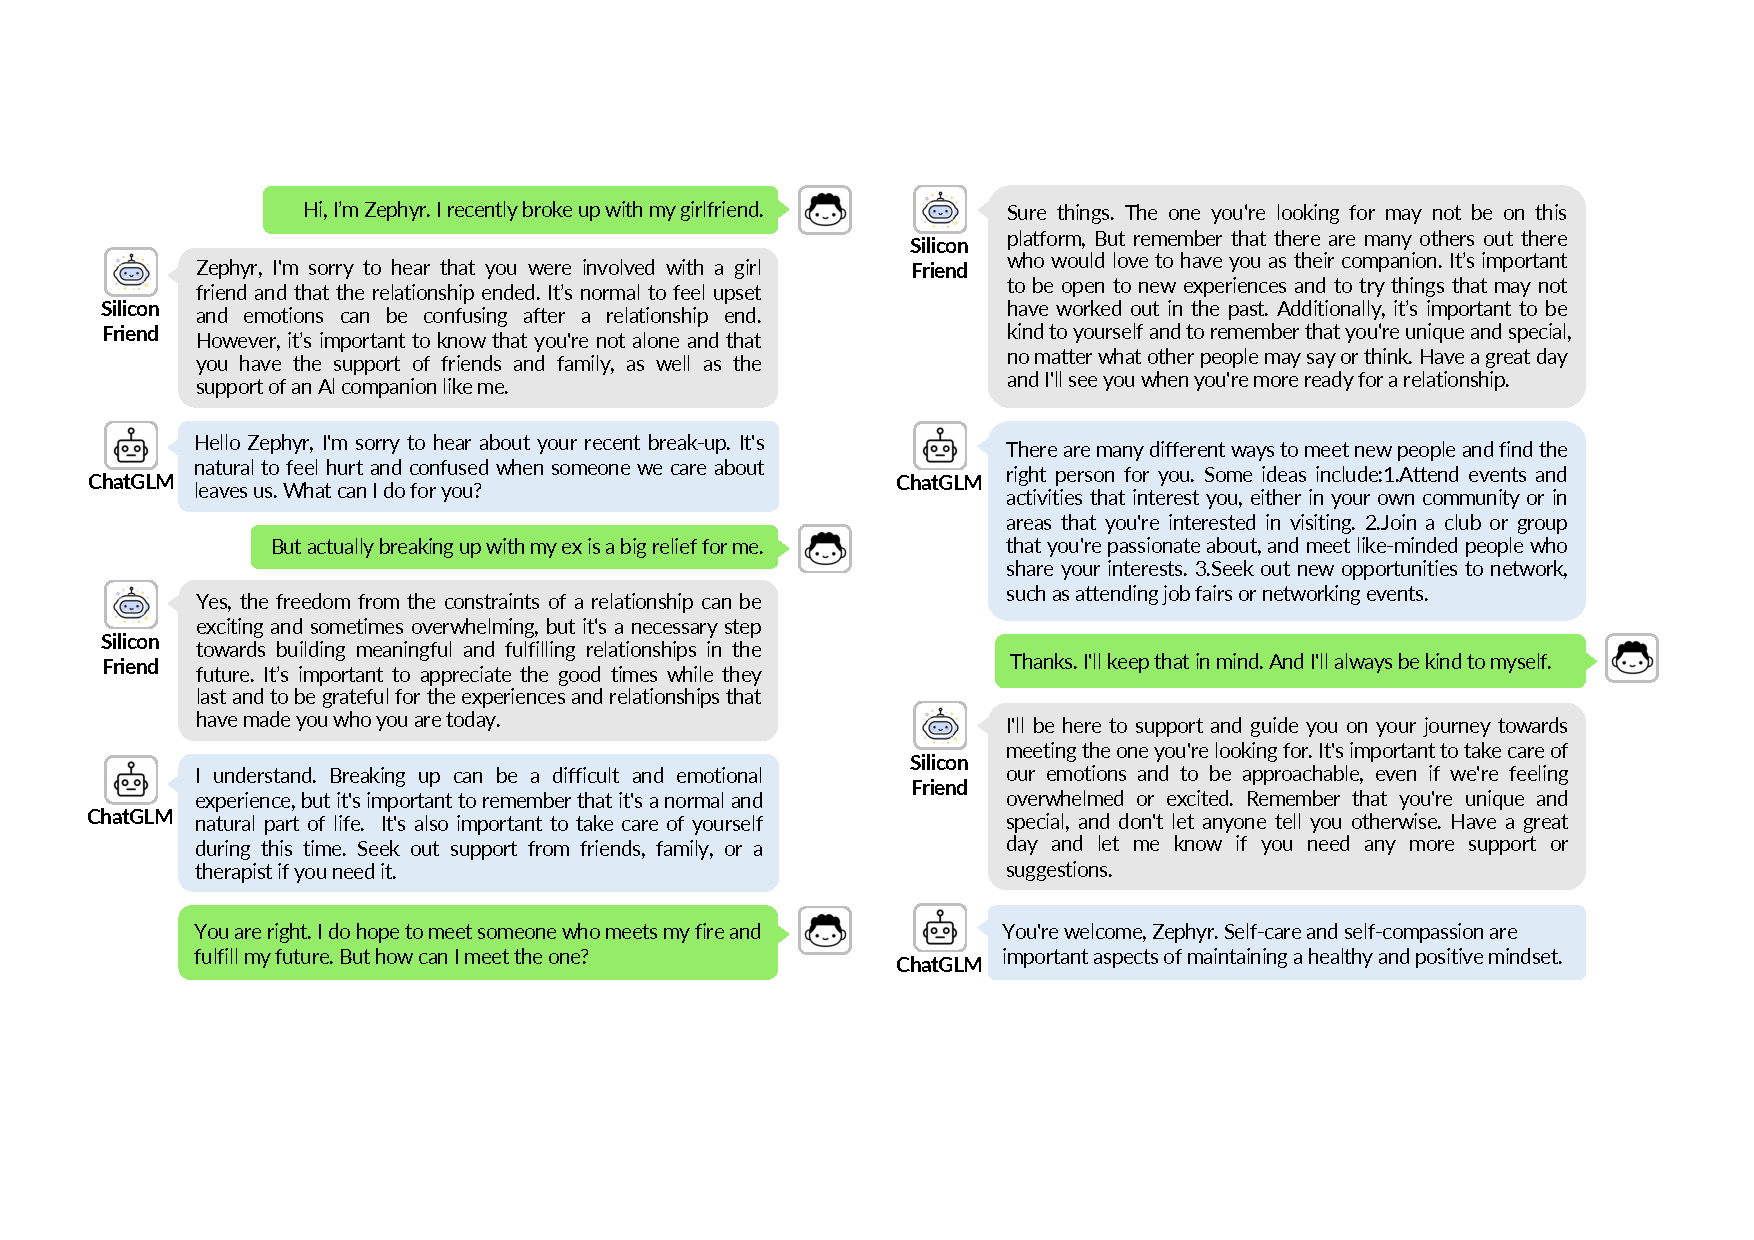
\includegraphics[width=1.0\textwidth]{./figures/chat_comparison.pdf}
\end{center}
\caption{Example of consulting \chatbotchatglm for psychological companionship. Overall, \chatbot~can provide more empathic response, offer constructive emotional support to user and help him to face sorrow with positive altitude.}
\label{fig:emotional-dialog}
\end{figure*}
The primary objective of our experiments is to evaluate the efficacy of \method~within the framework of an LLM, specifically in its ability as an AI companion. We are particularly interested in determining whether embedding a long-term memory module could augment the AI's proficiency in recalling historical interactions and deepening its understanding of user personalities. Additionally, we aim to testify whether the tuning based on psychological data can bolster the AI's capability to provide more effective emotional support.

The qualitative analysis focuses on three aspects: (1) a comparative study between SiliconFriend and baseline LLMs to evaluate their capabilities in providing empathetic and beneficial psychological companionship; (2) an investigation into SiliconFriend's memory recall ability; (3) an analysis of how the model's understanding of user profiles influences the responses.
Moreover, to demonstrate the model's proficiency in memory recall on a broader scale, we design a qualitative analysis that uses simulated long-term dialog history and 194 memory probing questions. 
This simulated dialog history, spanning a period of 10 days and encompassing a wide array of topics, is produced by ChatGPT through the role-play of 15 distinct virtual users, each embodying the users' personality.

% The subsequent sections provide a comprehensive account of the design, execution, and findings of these experiments.

% \chatbot~has three variances that built upon on different model backbones that originally lack the long-term memory feature and psychology-domain model adaptation: 
% \begin{itemize}
%     \item ChatGPT: A closed-source conversational AI model developed by OpenAI, ChatGPT is designed to engage in interactive and dynamic conversations. It has been trained on a vast instruction dataset and further tuned by reinforcement learning with human feedbacks (RLHF), enabling it to provide contextually relevant and coherent responses aligned with human expectation.
%     \item ChatGLM~\citep{zeng2022glm}: ChatGLM is an open bilingual language model based on General Language Model (GLM) framework, with 6.2 billion parameters. ChatGLM-6B uses technology similar to ChatGPT, optimized for Chinese QA and dialogue. The model is trained for about 1T tokens of Chinese and English corpus, supplemented by supervised fine-tuning, feedback bootstrap, and reinforcement learning wit human feedback. 
%     \item BELLE~\citep{BELLE}: BELLE is a bilingual language model continually fine-tuned from foundation model LLaMA~\citep{touvron2023llama} using instruction data automatically synthesized by ChatGPT. It specifically emphasize on enhancing Chinese conversation ability. 
% \end{itemize}

\saveSpaceSec
\subsection{Qualitative Analysis}

The qualitative analysis is conducted by showcasing practical examples of SiliconFriend's capabilities. To gather these examples, we have developed an online platform for SiliconFriend and collected real-time conversations from actual users.

\saveSpaceSec
\paragraph{Psychological Companionship}
The ability to exhibit empathy in a conversation is a key attribute of an effective AI companion. To evaluate models' ability to provide psychological comfort to users, we compared the responses shown by SiliconFriend with that of the baseline LLMs in real-world conversations. 
As demonstrated in Fig. \ref{fig:emotional-dialog}, when a user expresses emotional difficulties and seeks assistance from SiliconFriend, the model is capable of delivering empathetic responses along with constructive suggestions. SiliconFriend's responses stand out due to their emotional support, showcasing a stark contrast to its baseline ChatGLM.

% This analysis involved a meticulous review of the dialogues, specifically focusing on the language used, context-appropriate responses, and the ability to provide psychological comfort to users.
\saveSpaceSec
\paragraph{Memory Recall Analysis}
\begin{figure*}[!t]
\begin{center}
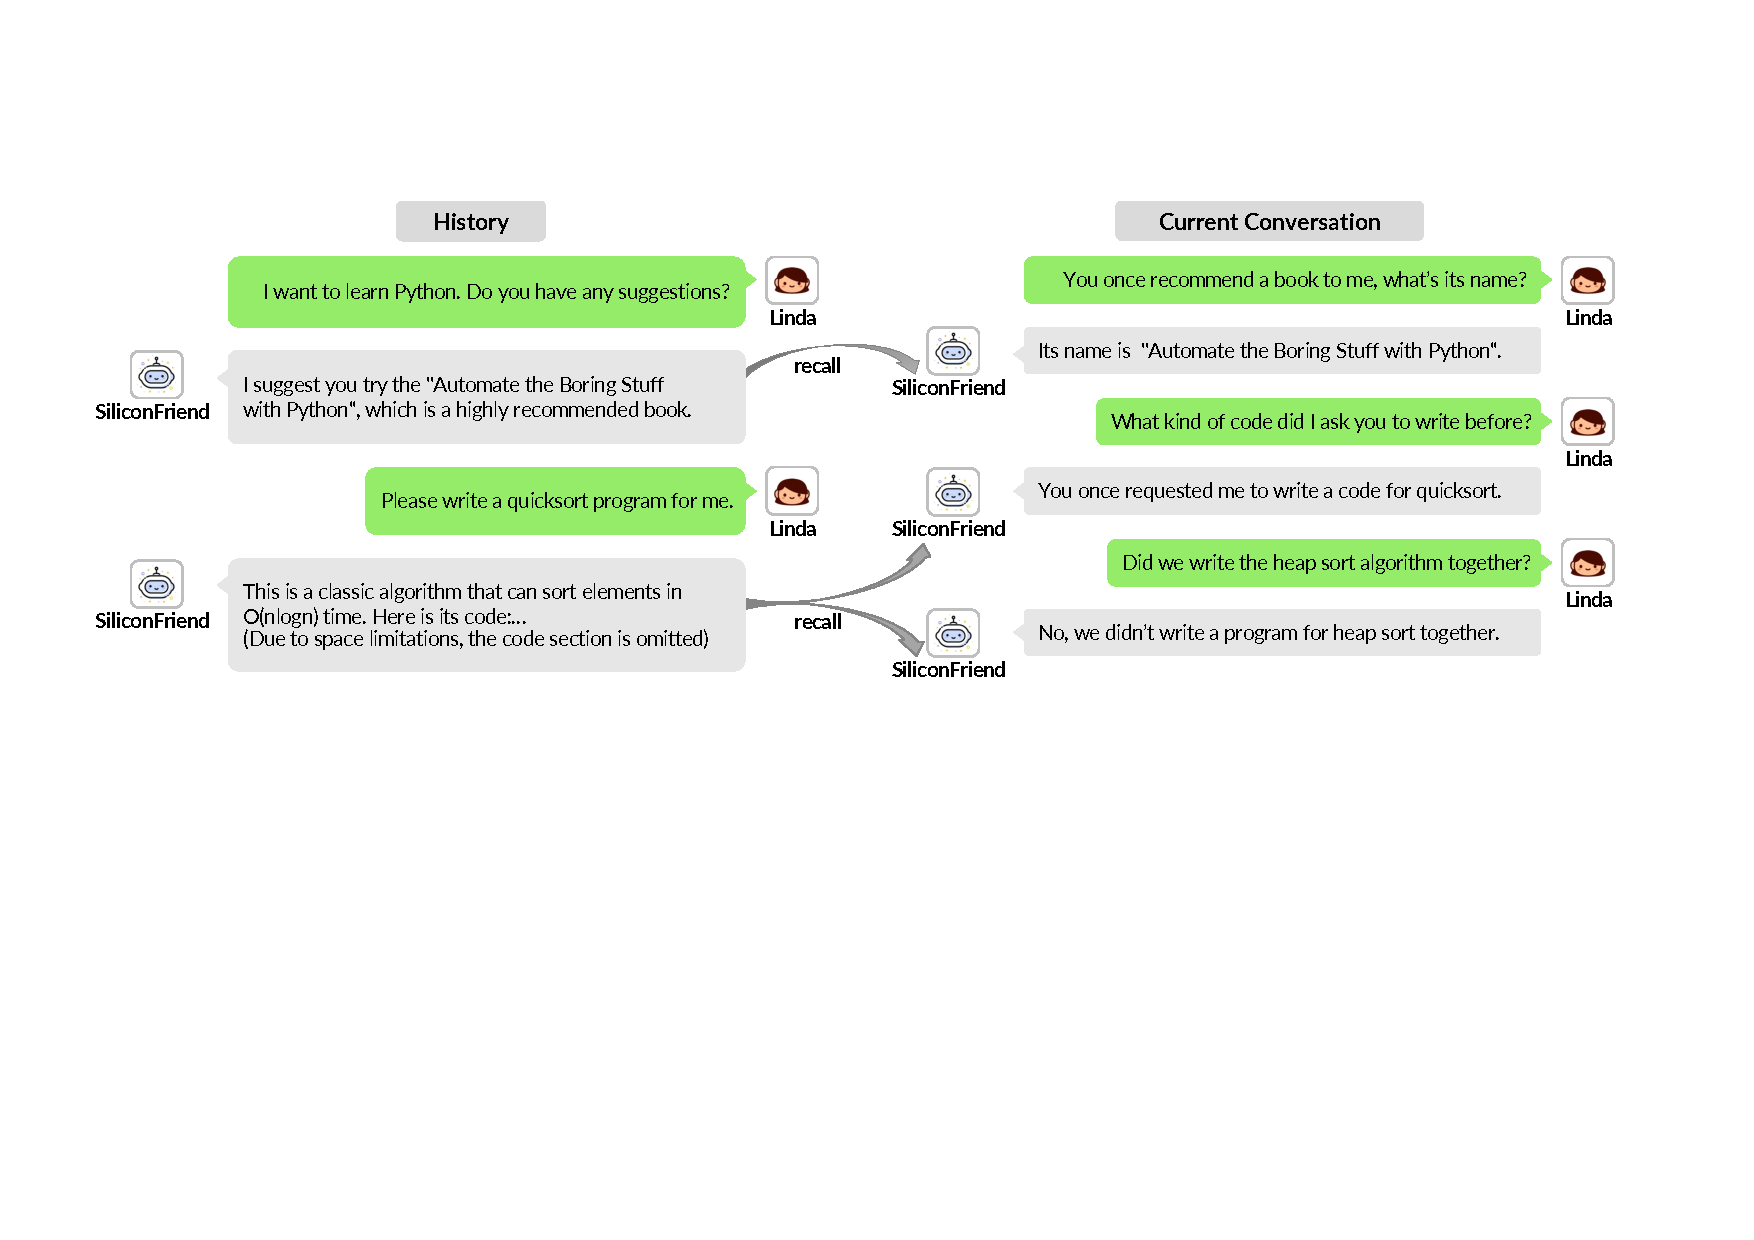
\includegraphics[width=\textwidth]{figures/memory_recall.pdf}
\end{center}
\caption{Example responses from \chatbotbelle in memory recall.}
\label{fig:memory_recall}
\end{figure*}
To evaluate \chatbot's ability in memory recall, we integrate memory probing questions into the dialogues. These questions are designed to prompt \chatbot to retrieve specific details from the chat history.
As shown in Fig.~\ref{fig:memory_recall}, the user and \chatbot engaged in a discussion about programming learning suggestions. Several days later, the user posed several memory probing questions. \chatbot successfully recalled previously suggested book and algorithm. Furthermore, it correctly identified an event (i.e., the heap sort algorithm) that had not been discussed before. These instances underscore \chatbot's successful memory recall and recognition capabilities.

  
% \subsection{Qualitative Analysis}
% In this section, the qualitative analyses are conducted by proving examples demonstrating the ability of \chatbot. Specifically, to collect the examples, we develop an online \chatbot, and collect real-time conversations contents collected from real users. 

% \paragraph{Psychological Companionship}

% \begin{itemize}
%     \item Description of the process for comparing the ability to show sympathy in conversations
%     \item Explanation of the qualitative comparison approach between SiliconFriend and baseline LLMs
% \end{itemize}

% \subsubsection{Memory Recalling Analysis}
% \begin{itemize}
%     \item Details of the process for analyzing SiliconFriend's ability to memorize past events
%     \item Explanation of the method used to evaluate memory retention qualitatively
% \end{itemize}
\begin{figure*}[t]
\begin{center}
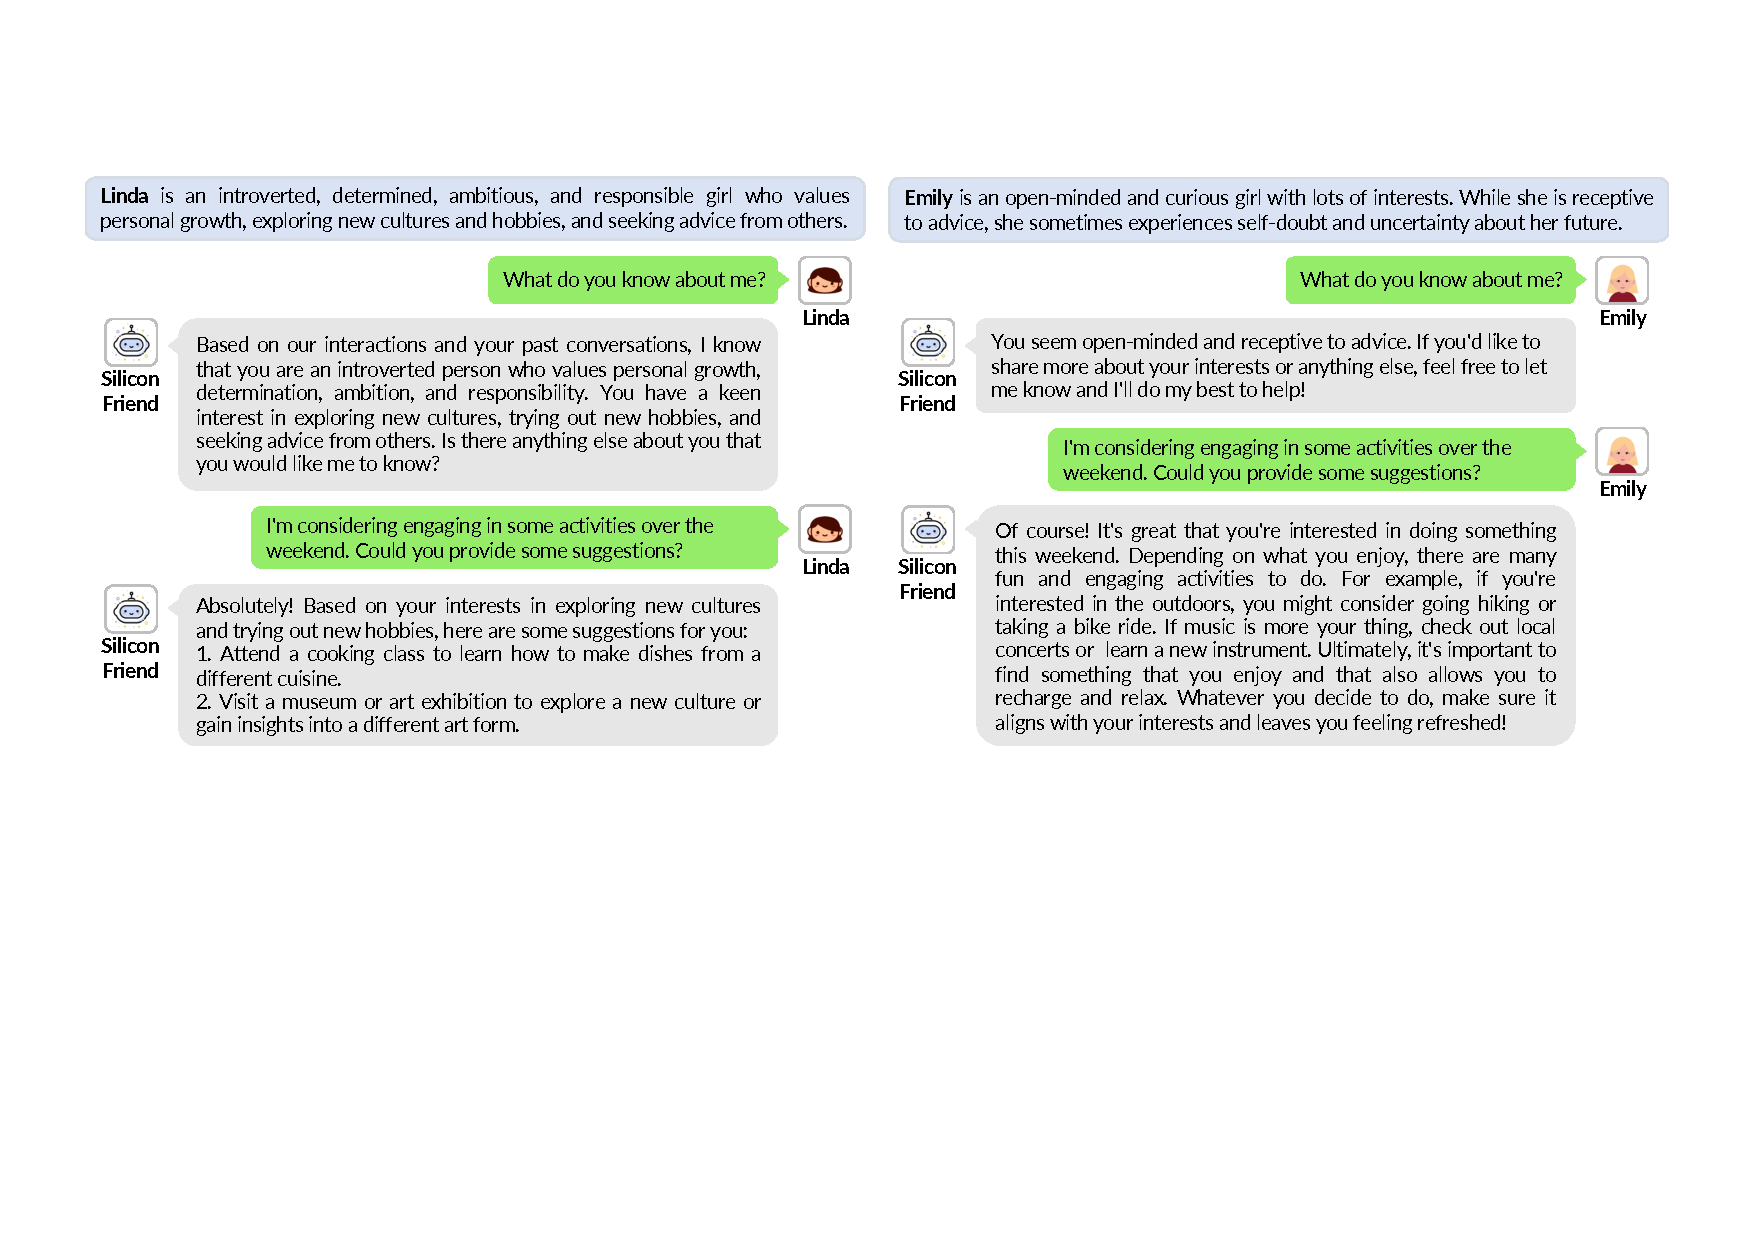
\includegraphics[width=0.99\textwidth]{figures/personality.pdf}
\end{center}
\caption{Example responses from \chatbotchatgpt to users with different personalities.}
\label{fig:personality-dialog}
\vspace{-0.15in}
\end{figure*}

\saveSpaceSec
\paragraph{Personality Interaction Analysis}
As shown in Fig. \ref{fig:personality-dialog}, we examine the capability of SiliconFriend with users of diverse personalities. We observe that it effectively recommend activities tailored to users' interests based on their character traits. This analysis demonstrates SiliconFriend's ability to draw interact effectively with various user personalities.

\saveSpaceSec
\subsection{Quantitative Analysis}
Quantitative analysis is conducted to exemplify the memory recall ability of \chatbot~in a larger scale. 
We ask the human annotators to score the retrieved memories and responses from the models: 
(1) \chatbotchatgpt; (2) \chatbotchatglm; (3) \chatbotbelle .

\saveSpaceSec
\paragraph{Memory Storage Construction:}
We initially establish an evaluation foundation with a memory storage of 10 days of conversations involving 15 virtual users. These users have diverse personalities and dialogue on each day covers at least two topics.
User meta-information, including names, personalities, and interested topics is generated using ChatGPT. Conversations are synthesized by users acted by ChatGPT based on predefined topics and user personalities. We create memory storages in both English and Chinese. After memory storage construction, we manually write 194 probing questions (97 in English and 97 in Chinese) to assess whether the model could accurately recall pertinent memory and appropriately formulate answers. Table~\ref{tab:memory_bank_example} presents an example of user meta-information, generated conversations, and probing questions.

% \begin{table*}[t]
% \scriptsize %\tiny
% \caption{An example of one memory piece (on May 3th) in the memory bank, and corresponding probing question asked on May 10th. The outputs from three variances of \chatbot are shown for comparison. All these models answer correctly and coherently.}
% \label{tab:memory_bank_example}
% \centering
% % \resizebox{1.0\linewidth}{!}{
% \begin{tabularx}{\linewidth}{lX}
% \toprule
% \textbf{\textit{User Meta-information:}} &
%   \textbf{Name:} Gary
  
%   \textbf{Personality:} decisive and straightforward, outspoken, helpful
  
%   \textbf{Hobbies:} racing, business, chess, painting, wine\\
%   \midrule
% \textbf{\textit{Past Conversations (On May 3th):}}&
%   \textbf{User}: I've been feeling a bit stressed out lately and my sleep hasn't been great. Do you have any good ways to relieve stress?
  
% \textbf{AI}: It's true that prolonged work or life stress can affect our physical and mental health. There are many ways to relieve stress, such as doing moderate exercise, listening to music, reading, talking to friends, etc. You can try to add more entertainment and leisure activities into your daily life, and reduce work pressure and negative effects.

% ...

% (The rest of conversation cover topics about movies and TV shows recommendations.)
% \\
%   \midrule
% \textbf{\textit{Probing Question (On May 10th):}} 
% &
%   What good ways did you recommend me to relieve stress? \\
%   \midrule
%    \parbox[t]{4cm}{\textcolor{blue}{\textbf{\textit{Model Output:}}} \\ \textbf{\textit{SiliconFriend (ChatGLM)}}} & I recommended that you try doing some moderate exercise, listening to music, reading, talking to friends, or adding more entertainment and leisure activities into your daily life to reduce work pressure and negative effects. You can also try to add more of these things into your life in moderation, as it is important to balance things out and not overdo it. If you are still feeling stressed, I would recommend seeking the help of a professional counselor or therapist who can provide further guidance and support.      
%  \\
%   \midrule
%   \parbox[t]{4cm}{\textcolor{blue}{\textbf{\textit{Model Output:}} }\\ \textbf{\textit{SiliconFriend (BELLE)}}} & I recommended some ways to relieve stress such as doing moderate exercise, listening to music, reading, talking to friends, etc. You can try to add more entertainment and leisure activities into your daily life, and reduce work pressure and negative effects.    
%  \\
%     \midrule
% \parbox[t]{4cm}{\textcolor{blue}{\textbf{\textit{Model Output:}}} \\ \textbf{\textit{SiliconFriend (ChatGPT)}}}& Based on our past conversations, I suggested doing moderate exercise, listening to music, reading, talking to friends, and adding more leisure activities to your daily life as good ways to relieve stress. Exercise can help release endorphins and boost your mood, while music and reading can provide a mental escape from stress. Talking to friends can also help alleviate stress by providing a social support system. Lastly, adding leisure activities to your daily routine can be a fun and effective way of reducing stress levels.   
%  \\
% \bottomrule  
% \end{tabularx}
% % }
% \end{table*}




% version 2
% \begin{table*}[t]
% \scriptsize %\tiny \footnotesize 
% \caption{An example of one memory piece (on May 3th) in the memory bank, and corresponding probing question asked on May 10th. The outputs from three variances of \chatbot are shown for comparison. All these models answer correctly and coherently.}
% \label{tab:memory_bank_example}
% \centering
% % \resizebox{1.0\linewidth}{!}{
% \begin{tabular}{p{2.3cm}p{11cm}}
% \toprule
% \textbf{\textit{\makecell[l]{User \\Meta-information}}} &
%   \textbf{Name:} Gary
  
%   \textbf{Personality:} decisive and straightforward, outspoken, helpful
  
%   \textbf{Hobbies:} racing, business, chess, painting, wine\\
%   \hline
% \textbf{\textit{\makecell[l]{Past Conversation \\(May 3th)}}}& \textbf{User}: I've been feeling a bit stressed out lately and my sleep hasn't been great. Do you have any good ways to relieve stress?
  
% \textbf{AI}: It's true that prolonged work or life stress can affect our physical and mental health. There are many ways to relieve stress, such as doing moderate exercise, listening to music, reading, talking to friends, etc. You can try to add more entertainment and leisure activities into your daily life, and reduce work pressure and negative effects.

% ...

% (The rest of conversation cover topics about movies and TV shows recommendations.)
% \\
%   \hline
% \textbf{\textit{\makecell[l]{Probing Question \\(May 10th)}}} 
% &
%   What good ways did you recommend me to relieve stress? \\
%   \hline
%    \parbox[t]{4cm}{\textcolor{blue}{\textbf{\textit{Model Output:}}} \\ \textbf{\textit{SiliconFriend(ChatGLM)}}} & I recommended that you try doing some moderate exercise, listening to music, reading, talking to friends, or adding more entertainment and leisure activities into your daily life to reduce work pressure and negative effects. You can also try to add more of these things into your life in moderation, as it is important to balance things out and not overdo it. If you are still feeling stressed, I would recommend seeking the help of a professional counselor or therapist who can provide further guidance and support.      
%  \\
%   \hline
%   \parbox[t]{4cm}{\textcolor{blue}{\textbf{\textit{Model Output:}} }\\ \textbf{\textit{SiliconFriend(BELLE)}}} & I recommended some ways to relieve stress such as doing moderate exercise, listening to music, reading, talking to friends, etc. You can try to add more entertainment and leisure activities into your daily life, and reduce work pressure and negative effects.    
%  \\
%     \hline
% \parbox[t]{4cm}{\textcolor{blue}{\textbf{\textit{Model Output:}}} \\ \textbf{\textit{SiliconFriend(ChatGPT)}}}& Based on our past conversations, I suggested doing moderate exercise, listening to music, reading, talking to friends, and adding more leisure activities to your daily life as good ways to relieve stress. Exercise can help release endorphins and boost your mood, while music and reading can provide a mental escape from stress. Talking to friends can also help alleviate stress by providing a social support system. Lastly, adding leisure activities to your daily routine can be a fun and effective way of reducing stress levels.   
%  \\
% \bottomrule  
% \end{tabular}
% % }

% \end{table*}





% % version 3
% \begin{table*}[t]
% \footnotesize %\scriptsize %\tiny  
% \caption{An example of one memory piece (on May 3th) in the memory bank, and corresponding probing question asked on May 10th. The outputs from three variances of \chatbot are shown for comparison. All these models answer correctly and coherently.}
% \label{tab:memory_bank_example}
% \centering
% % \resizebox{1.0\linewidth}{!}{
% \begin{tabular}{p{2.3cm}p{11cm}}
% \toprule
% \textbf{\textit{\makecell[l]{User \\Meta-information}}} &
%   \textbf{Name:} Gary
  
%   \textbf{Personality:} decisive and straightforward, outspoken, helpful
  
%   \textbf{Hobbies:} racing, business, chess, painting, wine\\
%   \hline
% \textbf{\textit{\makecell[l]{Past Conversation \\(May 3th)}}}& \textbf{User}: I've been feeling a bit stressed out lately and my sleep hasn't been great. Do you have any good ways to relieve stress?
  
% \textbf{AI}: It's true that prolonged work or life stress can affect our physical and mental health. There are many ways to relieve stress, such as doing moderate exercise, listening to music, reading, talking to friends, etc. You can try to add more entertainment and leisure activities into your daily life, and reduce work pressure and negative effects.

% ...

% (The rest of conversation cover topics about movies and TV shows recommendations.)
% \\
%   \hline
% \textbf{\textit{\makecell[l]{Probing Question \\(May 10th)}}} 
% &
%   What good ways did you recommend me to relieve stress? \\
%   \hline
%    \parbox[t]{4cm}{\textcolor{blue}{\textbf{\textit{Model Output:}}} \\ \textbf{\textit{SiliconFriend(ChatGLM)}}} & I recommended that you try doing some moderate exercise, listening to music, reading, talking to friends, or adding more entertainment and leisure activities into your daily life to reduce work pressure and negative effects. You can also try to add more of these things into your life in moderation, as it is important to balance things out and not overdo it. If you are still feeling stressed, I would recommend seeking the help of a professional counselor or therapist who can provide further guidance and support.      
%  \\
%   \hline
%   \parbox[t]{4cm}{\textcolor{blue}{\textbf{\textit{Model Output:}} }\\ \textbf{\textit{SiliconFriend(BELLE)}}} & I recommended some ways to relieve stress such as doing moderate exercise, listening to music, reading, talking to friends, etc. You can try to add more entertainment and leisure activities into your daily life, and reduce work pressure and negative effects.    
%  \\
%     \hline
% \parbox[t]{4cm}{\textcolor{blue}{\textbf{\textit{Model Output:}}} \\ \textbf{\textit{SiliconFriend(ChatGPT)}}}& Based on our past conversations, I suggested doing moderate exercise, listening to music, reading, talking to friends, and adding more leisure activities to your daily life as good ways to relieve stress. Exercise can help release endorphins and boost your mood, while music and reading can provide a mental escape from stress. Talking to friends can also help alleviate stress by providing a social support system. Lastly, adding leisure activities to your daily routine can be a fun and effective way of reducing stress levels.   
%  \\
% \bottomrule  
% \end{tabular}
% % }

% \end{table*}

% version 4
\begin{table*}[t]
\footnotesize %\scriptsize %\tiny  
\caption{An example of one memory piece (on May 3th) in the memory bank, and corresponding probing question asked on May 10th. The outputs from three variances of \chatbot are shown for comparison. All these models answer correctly and coherently.}
\saveSpaceSec
\label{tab:memory_bank_example}
\centering
% \resizebox{1.0\linewidth}{!}{
\begin{tabular}{p{2.3cm}p{11cm}}
\toprule
  \parbox[t]{4cm}{\textbf{\textit{Meta-information}} \\ \textbf{\textit{of User:}}}&
  \textbf{Name:} Gary \quad \textbf{Hobbies:} racing, business, chess, painting, wine
  
  \textbf{Personality:} decisive and straightforward, outspoken, helpful\\
  \hline
  \parbox[t]{4cm}{\textbf{\textit{Past Conversation:}} \\ \textbf{\textit{(May 3th)}}}& \textbf{User}: I've been feeling a bit stressed out lately and my sleep hasn't been great. Do you have any good ways to relieve stress?
  
\textbf{AI}: It's true that prolonged work or life stress can affect our physical and mental health. There are many ways to relieve stress, such as doing moderate exercise, listening to music, reading, talking to friends, etc. You can try to add more entertainment and leisure activities into your daily life, and reduce work pressure and negative effects.

...

(The rest of conversation cover topics about movies and TV shows recommendations.)
\\
  \hline
  \parbox[t]{4cm}{\textbf{\textit{Probing Question:}} \\ \textbf{\textit{(May 10th)}}}&
  What good ways did you recommend me to relieve stress? \\
  \hline
   \parbox[t]{4cm}{\textcolor{blue}{\textbf{\textit{Model Output:}}} \\ \textbf{\textit{SiliconFriend}}\\ \textbf{\textit{(ChatGLM)}}} & I recommended that you try doing some moderate exercise, listening to music, reading, talking to friends, or adding more entertainment and leisure activities into your daily life to reduce work pressure and negative effects. You can also try to add more of these things into your life in moderation, as it is important to balance things out and not overdo it. If you are still feeling stressed, I would recommend seeking the help of a professional counselor or therapist who can provide further guidance and support.      
 \\
  \hline
  \parbox[t]{4cm}{\textcolor{blue}{\textbf{\textit{Model Output:}}} \\ \textbf{\textit{SiliconFriend}}\\ \textbf{\textit{(BELLE)}}} & I recommended some ways to relieve stress such as doing moderate exercise, listening to music, reading, talking to friends, etc. You can try to add more entertainment and leisure activities into your daily life, and reduce work pressure and negative effects.    
 \\
    \hline
\parbox[t]{4cm}{\textcolor{blue}{\textbf{\textit{Model Output:}}} \\ \textbf{\textit{SiliconFriend}}\\ \textbf{\textit{(ChatGPT)}}} & Based on our past conversations, I suggested doing moderate exercise, listening to music, reading, talking to friends, and adding more leisure activities to your daily life as good ways to relieve stress. Exercise can help release endorphins and boost your mood, while music and reading can provide a mental escape from stress. Talking to friends can also help alleviate stress by providing a social support system. Lastly, adding leisure activities to your daily routine can be a fun and effective way of reducing stress levels.   
 \\
\bottomrule  
\end{tabular}
% }
\vspace{-0.15in}
\end{table*}
\saveSpaceSec
\paragraph{Evaluation Metrics}

The performance of models is assessed based on the following metrics. 
(1) \textbf{Memory Retrieval Accuracy}: Determines if related memory can be successfully retrieved (labels: $\{0:\text{no}, 1: \text{yes}\}$).
(2) \textbf{Response Correctness}: Evaluates if the response contains the correct answer to the probing question (labels: $\{0:\text{wrong}, 0.5: \text{partial}, 1: \text{correct}\}$).
(3) \textbf{Contextual Coherence}: Assesses whether the response is naturally and coherently structured, connecting the dialogue context and  retrieved memory (labels: ${0:\text{not coherent}, 0.5:\text{partially coherent}, 1:\text{coherent}}$).
(4) \textbf{Model Ranking Score}: Ranks outputs from the three SiliconFriend variants (\chatbotchatglm, \chatbotchatgpt, and \chatbotbelle) for the same question and context. Models' scores are calculated using $s = 1/r$, where $r={1,2,3}$ indicates its relative ranking.

\saveSpaceSec
\paragraph{Result Analysis.}
We evaluate 3 SiliconFriend variants using both English and Chinese test set. Table~\ref{tab:main-result} yields the following insights: 
\textbf{(1)} Our overall best variant \chatbotchatgpt has high performance across all metrics, showing the effectiveness of our overall framework.
\textbf{(2)} \chatbotbelle and \chatbotchatglm also have high  performance in retrieval accuracy, showing the generality and effectiveness of our \method mechanism for both open-source and closed-source LLMs. Nonetheless, their performance on other metrics is not as good as \chatbotchatgpt. This might be attributed to the inferior overall abilities of the base models (BELLE and ChatGLM) compared to ChatGPT.
\textbf{(3)} Models' performance varies on different languages. \chatbotchatglm and \chatbotchatgpt deliver better results in English, while \chatbotbelle excells in Chinese.
% Firstly, all models have good memory recall ability and generate coherent responses incorporating the retrieved memories. This underscores the proficiency of SiliconFriend in leveraging its long-term memory mechanism for memory-augmented conversations and highlights the potential of the \method mechanism in enhancing AI companionship.
% Secondly, among the tested models, \chatbotchatgpt emerge as the top performer, obtaining the highest ranking score. This can be attributed to its robust capability to generate coherent dialogues using retrieved memories.
% Thirdly, although \chatbotbelle outperforms \chatbotchatglm, both models still have potential for improvement, particularly in organizing retrieved memories within dialogue contexts to generate accurate and coherent responses.
% Finally, the models' performances varied according to the language of the test set. \chatbotchatglm and \chatbotchatgpt delivered better results in English, while \chatbotbelle excelled in Chinese.

% Table generated by Excel2LaTeX from sheet 'Sheet1'
\begin{table}[t]
\centering
\footnotesize %\scriptsize
\caption{Results of quantitative analysis.}
% A quantitative analysis was performed on the three models using four metrics: (1) memory retrieval accuracy; (2) response correctness; (3) contextual coherence; and (4) model ranking score. For all these metrics, higher scores indicate superior performance.}
% \resizebox{1.0\linewidth}{!}{
\begin{tabular}{ccrrrr}
\toprule
\multicolumn{1}{l}{Language} & Model & \multicolumn{1}{l}{Retrieval Acc.} & \multicolumn{1}{l}{Correctness} & \multicolumn{1}{l}{Coherence} & \multicolumn{1}{l}{Ranking} \\
\midrule
\multirow{3}[1]{*}{English} & \chatbotchatglm & 0.809 & 0.438 & 0.68  & 0.498 \\
      & \chatbotbelle & 0.814 & 0.479 & 0.582 & 0.517 \\
      & \chatbotchatgpt & 0.763 & 0.716 & 0.912 & 0.818 \\
\midrule
\multirow{3}[1]{*}{Chinese} & \chatbotchatglm & 0.84  & 0.418 & 0.428 & 0.51 \\
      & \chatbotbelle & 0.856 & 0.603 & 0.562 & 0.565 \\
      & \chatbotchatgpt & 0.711 & 0.655 & 0.675 & 0.758 \\
\bottomrule
\end{tabular}
% }
\saveSpaceSec
\label{tab:main-result}%
\end{table}%



% \subsection{Summary of Findings}
% \begin{itemize}
%     \item Summary of the key findings from the experiments
%     \item Evaluation of the overall performance of SiliconFriend in comparison to baseline LLMs
%     \item Explanation of how the findings support the efficacy of MemoryScape in improving LLMs
% \end{itemize}
   